\section{Backup}
\begin{frame}{Experiment 1, the line: RSSI, not distance, predicts the cost}
    \begin{columns}[T]
    \column{0.48\textwidth}
    \centering
    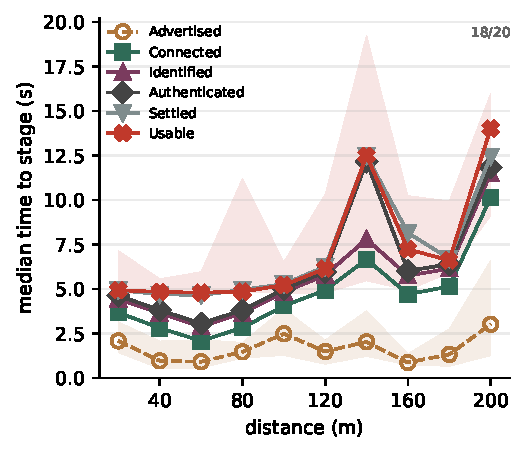
\includegraphics[width=\linewidth]{figures/line200_stages.pdf}
    \captionof{figure}{Time to link stage, by distance}
    \column{0.48\textwidth}
    \centering
    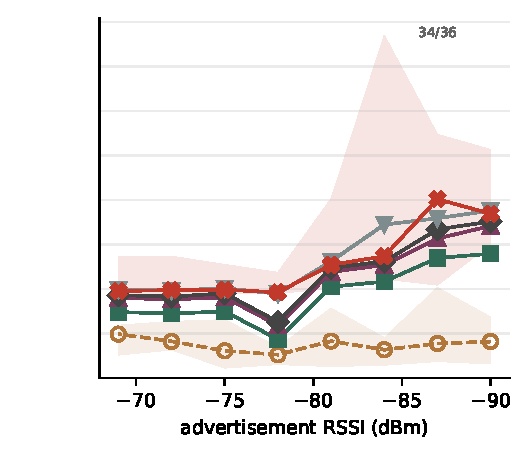
\includegraphics[width=\linewidth]{figures/line200_stages_vs_rssi.pdf}
    \captionof{figure}{The same runs, by RSSI}
    \end{columns}
    \begin{itemize}
        \item Discovery is quick and bound by the radio; identifying the peer is what costs. % 99 of 100 runs reached a session
        \item By distance the picture is confusing: RSSI values measured at different distances overlap
    \end{itemize}
    \takeaway{Pooled by RSSI, every stage rises monotonically.}
\end{frame}
\begin{frame}{Experiment 1, the line: delivery and acknowledgements}
    \begin{columns}[T]
    \column{0.48\textwidth}
    \centering
    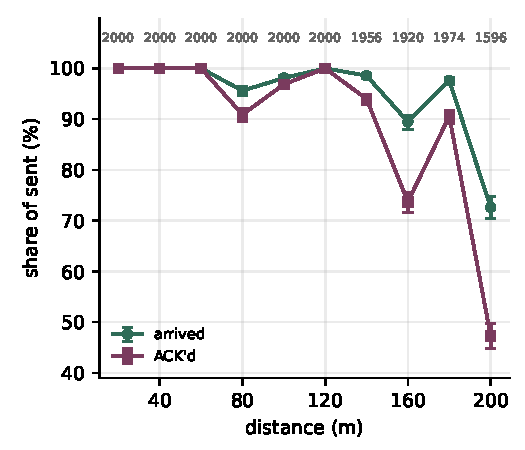
\includegraphics[width=\linewidth]{figures/line200_delivery_vs_distance.pdf}
    \captionof{figure}{Delivery and ACKs, by distance}
    \column{0.48\textwidth}
    \centering
    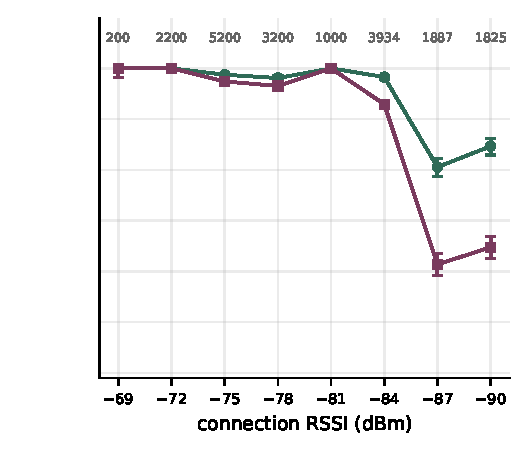
\includegraphics[width=\linewidth]{figures/line200_delivery_vs_rssi.pdf}
    \captionof{figure}{The same runs, by RSSI}
    \end{columns}
    \begin{itemize}
        \item Lossless above $-84$\,dBm%; beyond 120\,m the median ACK time climbs from 150\,ms to 3.1\,s
    \end{itemize}
    \takeaway{Judge links by RSSI.}
\end{frame}
\begin{frame}{Experiment 2, the diluting clique: custody does not rescue delivery}
    \begin{columns}[T]
    \column{0.56\textwidth}
    \centering
    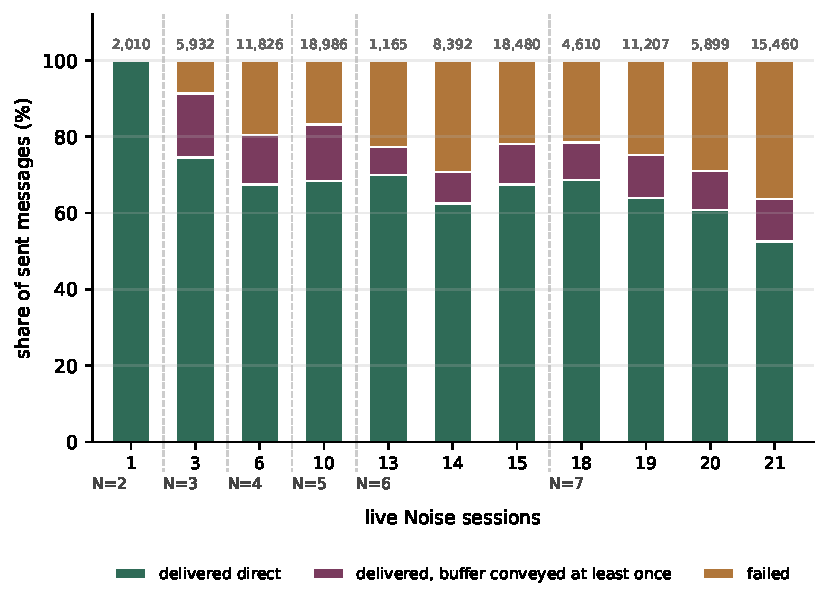
\includegraphics[width=\linewidth]{figures/clique_delivery_outcome_by_sessions.pdf}
    \captionof{figure}{Per-message outcome by live Noise sessions}
    \column{0.42\textwidth}
    \raggeditems
    \begin{itemize}
        \item Per message: delivered directly, conveyed from a peer's buffer, or failed
        \item Direct delivery drops to about 50\,\% at 21 live sessions; failures rise from 9\,\% to 37\,\%
        \item Conveyance covers only 5 to 10\,\% of deliveries
    \end{itemize}
    \end{columns}
    \takeaway{Greedy link establishment fails under contention: control plane link establishment needs a strategy.}
\end{frame}

\begin{frame}{Expriment3 the link-flap model in numbers}
    \begin{columns}[T]
    \column{0.52\textwidth}
    \centering
    \textbf{Nexus 5X link losses used by the simulator}\\[0.5ex]
    \small
    \begin{tabular}{@{}rrr@{}}
        \toprule
        links held $k$ & $\lambda(k)$ per node-minute & per link, $\lambda(k)/k$ \\
        \midrule
        1 & 1.13 & 1.13 \\
        2 & 1.13 & 0.57 \\
        3 & 1.18 & 0.39 \\
        4 & 1.36 & 0.34 \\
        5 & 1.28 & 0.26 \\
        6 & 1.44 & 0.24 \\
        7 & 1.57 & 0.22 \\
        \bottomrule
    \end{tabular}\\[1ex]
    {\footnotesize $k = 1$ was never observed and reuses the value of $k = 2$}
    \column{0.46\textwidth}
    \raggeditems
    \begin{itemize}
        \item The per-node rate rises mildly with $k$, while the per-link rate falls: a node with more links is not proportionally more fragile per link
        \item Every 30\,s each node draws a Poisson number of drops and picks the victim links uniformly
        \item Outage lengths are resampled from 1\,000 quantiles of the measured Nexus 5X outages: median 37\,s, mean 236\,s, maximum 5\,356\,s
        \item An exponential fit was rejected: too few short and too few very long outages
    \end{itemize}
    \end{columns}
\end{frame}

% \begin{frame}{Path loss along the line}
%     \centering
%     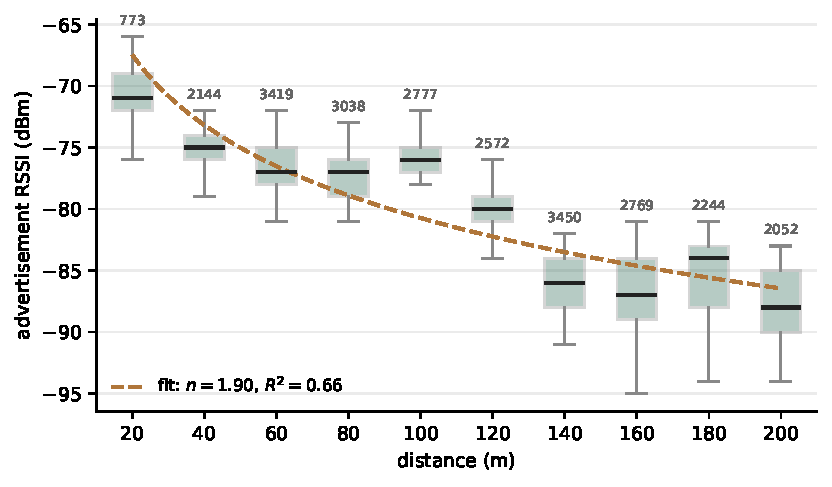
\includegraphics[width=0.66\textwidth]{figures/line200_path_loss.pdf}
%     \captionof{figure}{$\mathrm{RSSI}(d) \approx -43.5 - 18.8\log_{10} d$, a path-loss exponent of about 1.9, residual $\sigma = 3.6$\,dB, fitted on 34\,669 advertisement sightings at ten positions}
% \end{frame}

% \begin{frame}{Time to link stage by distance}
%     \begin{columns}[T]
%     \column{0.48\textwidth}
%     \centering
%     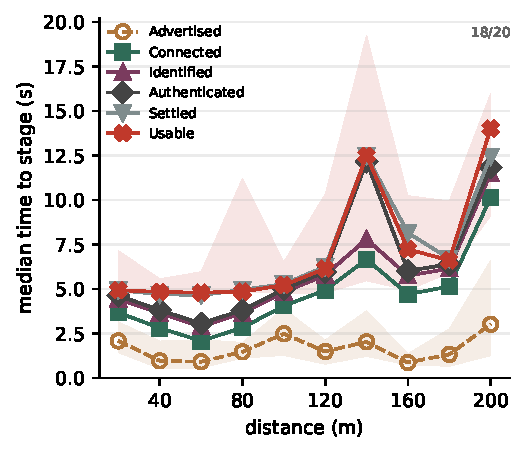
\includegraphics[width=\linewidth]{figures/line200_stages.pdf}
%     \captionof{figure}{Time to each link stage, by distance}
%     \column{0.5\textwidth}
%     \centering
%     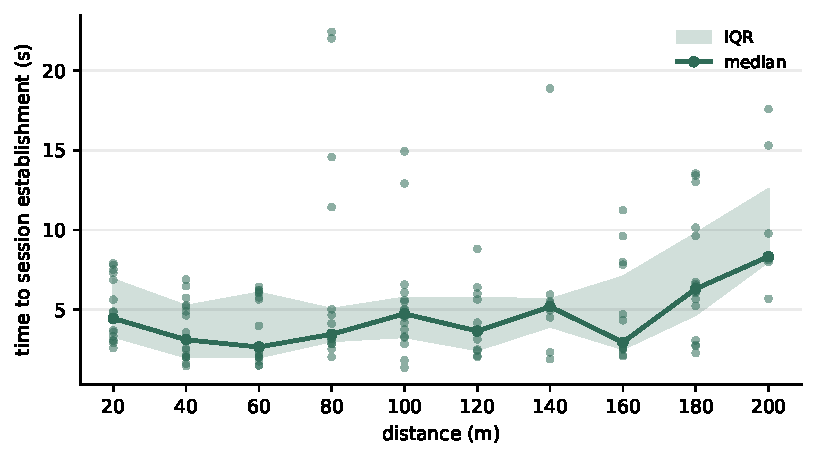
\includegraphics[width=\linewidth]{figures/line200_establishment_clean.pdf}
%     \captionof{figure}{Time to session, runs with GATT dial errors removed}
%     \end{columns}
%     \begin{itemize}
%         \item Hardware errors in the Bluetooth stack, especially around 140\,m, dominate the raw medians; removing those runs gives the expected upward trend
%     \end{itemize}
% \end{frame}

\begin{frame}{Delivery under load along the line}
    \centering
    \small
    \begin{tabular}{@{}rrrrrrr@{}}
        \toprule
        \textbf{d (m)} & \textbf{sent} & \textbf{arrived} & \textbf{acked} & \textbf{arrived} & \textbf{acked} & \textbf{ack p50} \\
        \midrule
         20 & 2000 & 2000 & 2000 & 100.0\,\% & 100.0\,\% &  123\,ms \\
         40 & 2000 & 2000 & 2000 & 100.0\,\% & 100.0\,\% &  133\,ms \\
         60 & 2000 & 2000 & 2000 & 100.0\,\% & 100.0\,\% &  135\,ms \\
         80 & 2000 & 1912 & 1818 &  95.6\,\% &  95.1\,\% &  150\,ms \\
        100 & 2000 & 1962 & 1937 &  98.1\,\% &  98.7\,\% &  144\,ms \\
        120 & 2000 & 2000 & 2000 & 100.0\,\% & 100.0\,\% &  166\,ms \\
        140 & 1956 & 1928 & 1838 &  98.6\,\% &  95.3\,\% &  380\,ms \\
        160 & 1920 & 1719 & 1415 &  89.5\,\% &  82.3\,\% & 1919\,ms \\
        180 & 1974 & 1929 & 1788 &  97.7\,\% &  92.7\,\% &  435\,ms \\
        200 & 1596 & 1161 &  755 &  72.7\,\% &  65.0\,\% & 3138\,ms \\
        \midrule
        all & 19446 & 18611 & 17551 & 95.7\,\% & 94.3\,\% & 154\,ms \\
        \bottomrule
    \end{tabular}\\[1ex]
    {\footnotesize 100 messages per trial per direction, both directions pooled; ack latency is the per-trial median of medians}
\end{frame}

% \begin{frame}{Control-plane bytes to reach each link stage}
%     \begin{columns}[T]
%     \column{0.42\textwidth}
%     \centering
%     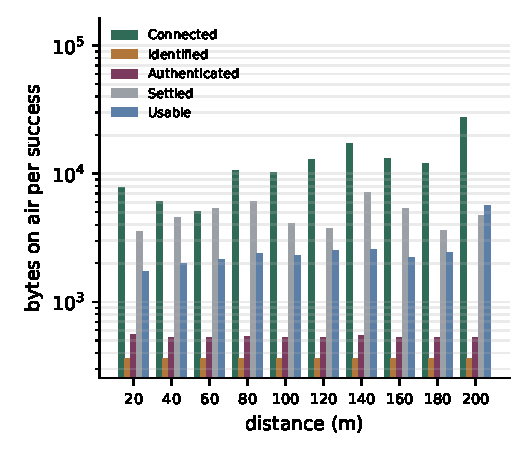
\includegraphics[width=\linewidth]{figures/line200_stage_bytes_rungs.pdf}
%     \captionof{figure}{Bytes to each link stage, by distance}
%     \column{0.42\textwidth}
%     \centering
%     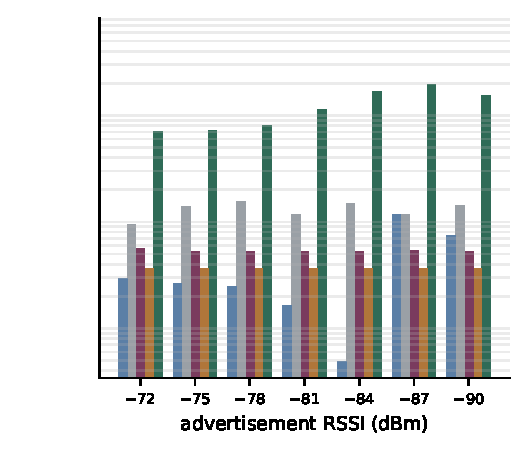
\includegraphics[width=\linewidth]{figures/line200_stage_bytes_rungs_rssi.pdf}
%     \captionof{figure}{Bytes to each link stage, by RSSI}
%     \end{columns}
%     \begin{itemize}
%         \item Establishing a GATT link costs 5 to 27\,kB of advertising at a 135\,ms interval
%         \item Identity costs 364 B (two ANNOUNCEs) and a session 524 B (four packets), whatever the RSSI
%     \end{itemize}
% \end{frame}

\begin{frame}{Delivery and latency along the line, by distance}
    \centering
    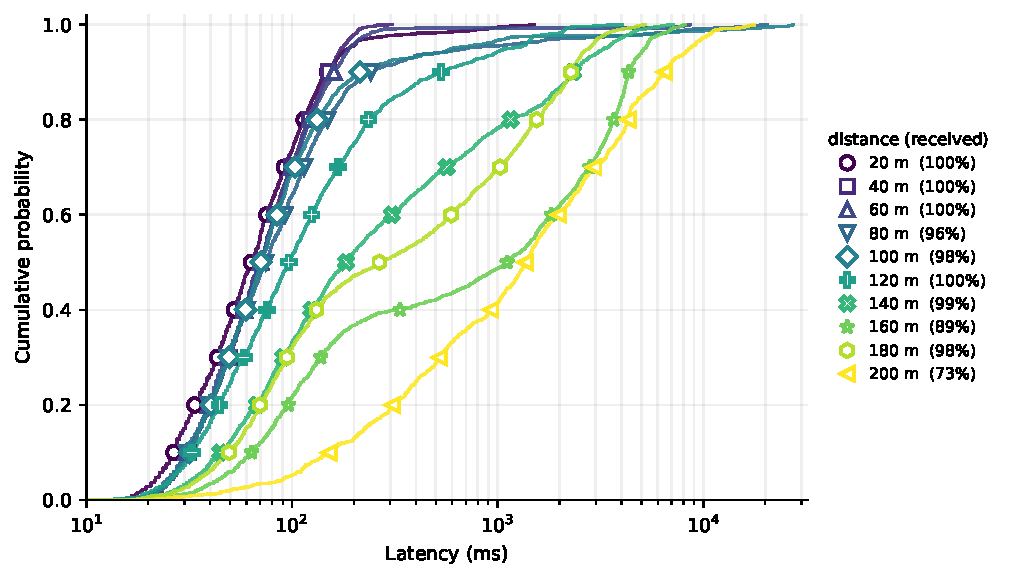
\includegraphics[width=\linewidth]{figures/line200_latency_cdf.pdf}
    \captionof{figure}{Message latency CDF, by distance}
\end{frame}

\begin{frame}{The diluting clique in numbers}
    \centering
    \small
    \setlength{\tabcolsep}{2.5pt}
    \begin{tabular}{@{}rrrrrrr@{}}
        \toprule
        \textbf{N} & \textbf{offered} & \textbf{sent} & \textbf{arrived} & \textbf{acked} & \textbf{lat p50} & \textbf{carried} \\
        \midrule
        2 &   6.7/s &  2000 & 100.0\,\% & 100.0\,\% & 0.11\,s &  0.0\,\% \\
        3 &  20.0/s &  5965 &  91.5\,\% &  79.5\,\% & 11.0\,s &  5.4\,\% \\
        4 &  40.0/s & 11940 &  80.3\,\% &  63.9\,\% & 31.6\,s & 10.1\,\% \\
        5 &  66.7/s & 19736 &  83.6\,\% &  75.1\,\% & 12.3\,s &  7.6\,\% \\
        6 & 100.0/s & 28793 &  75.7\,\% &  70.3\,\% &  8.3\,s &  6.5\,\% \\
        7 & 140.0/s & 38112 &  70.3\,\% &  57.8\,\% &  9.1\,s & 10.4\,\% \\
        \bottomrule
    \end{tabular}

    \vspace{1ex}
    {\footnotesize Ten trials per clique size, pooled over all senders; offered load in messages per second. \emph{Carried}: share of deliveries made out of a store-carry-forward buffer rather than over a live link.}
\end{frame}

\begin{frame}{Advertising cadence at idle}
    \centering
    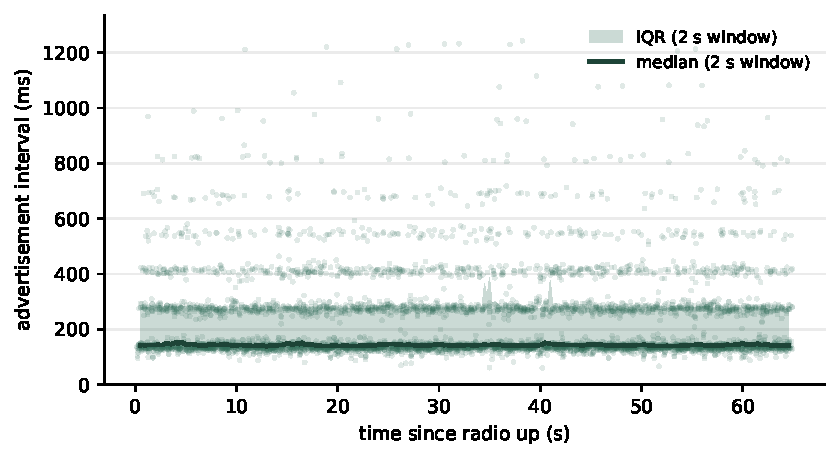
\includegraphics[width=0.8\textwidth]{figures/adv_interval_idle.pdf}
    \captionof{figure}{Median 7.41\,Hz, an advertisement interval of about 135\,ms, over twenty cold desk runs; even with an idle scanner roughly a third of the advertisements are not captured. Native stacks expose no callback for sent advertisements, so this baseline estimates the advertising bytes on the line.}
\end{frame}

\begin{frame}{Raw capacity of the two underlays on a Nexus 5X}
    \begin{columns}[T]
    \column{0.48\textwidth}
    \centering
    \textbf{BLE, one GATT link, 1\,m, write without response}\\[0.5ex]
    \small
    \begin{tabular}{@{}rrr@{}}
        \toprule
        Write size (B) & Writes/s & Delivered (kB/s) \\
        \midrule
        64  & 202 & 12.9 \\
        138 & 222 & 30.7 \\
        244 & 223 & 54.5 \\
        380 & 165 & 62.7 \\
        448 & 145 & 65.0 \\
        514 & 125 & 64.1 \\
        \bottomrule
    \end{tabular}\\[1ex]
    {\footnotesize The binding constraint is writes per second, not bytes offered; the ceiling is 63 to 65\,kB/s at the full 514-byte ATT payload}
    \column{0.48\textwidth}
    \centering
    \textbf{UDX, one isolate per stream}\\[0.5ex]
    \small
    \begin{tabular}{@{}rr@{}}
        \toprule
        Concurrent peers & Total throughput (bytes/s) \\
        \midrule
        1  & 628\,800 \\
        2  & 1\,321\,300 \\
        4  & 1\,952\,600 \\
        6  & 1\,634\,900 \\
        20 & 2\,459\,200 \\
        48 & 2\,406\,300 \\
        96 & 1\,757\,500 \\
        \bottomrule
    \end{tabular}\\[1ex]
    {\footnotesize About 2.4\,MB/s, the UDX capacity used by the \texttt{amigo-udx} arm}
    \end{columns}
\end{frame}

\begin{frame}{Buffer occupancy at scale}
    \centering
    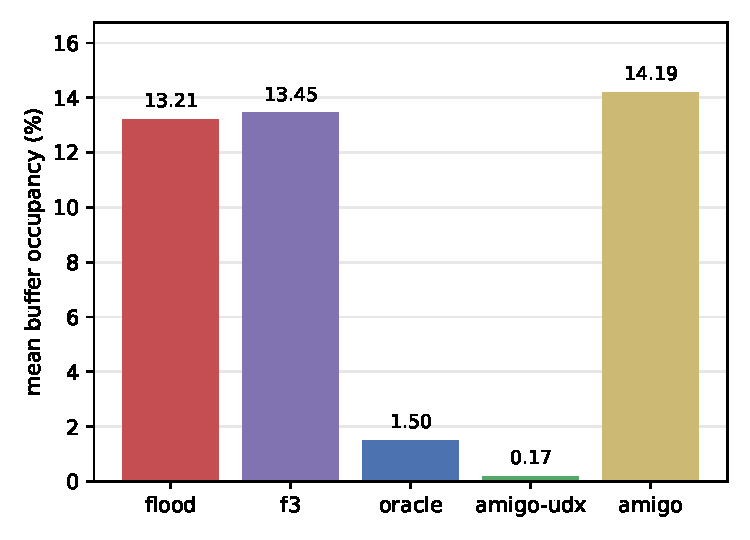
\includegraphics[width=0.66\textwidth]{figures/sim_buffer_occupancy.pdf}
    \captionof{figure}{Mean DTN buffer occupancy for the five arms at 392 nodes, 1\,msg/s network-wide, 25 seeded placements per arm. \texttt{amigo-udx} needs the least buffer; \texttt{f3} relays half as much as \texttt{flood} but buffers the same; \texttt{amigo} over BLE alone buffers the most.}
\end{frame}

\begin{frame}{Noise XX in three messages}
    \centering
    \begin{tikzpicture}[x=1mm,y=1mm, font=\small,
        note/.style={font=\footnotesize, text=black!65, text width=30mm},
        msg/.style={->, thick, TUMBlue}]
        \node[font=\small\bfseries] at (36,50) {Initiator $i$};
        \node[font=\small\bfseries] at (82,50) {Responder $r$};
        \draw[thick, black!60] (36,47) -- (36,2);
        \draw[thick, black!60] (82,47) -- (82,2);
        \draw[msg] (36,42) -- (82,40) node[midway, above=1.5pt, sloped] {1: \texttt{e}, cleartext, 115 B};
        \draw[msg] (82,29) -- (36,27) node[midway, above=1.5pt, sloped] {2: \texttt{e, ee, s, es}, 163 B};
        \draw[msg] (36,16) -- (82,14) node[midway, above=1.5pt, sloped] {3: \texttt{s, se}, 131 B};
        \node[note, anchor=east, align=right] at (34,42) {fresh ephemeral key $e_i$};
        \node[note, anchor=west, align=left] at (84,34) {fresh $e_r$; derive \texttt{ee}, \texttt{es}; send the static key $s_r$ encrypted};
        \node[note, anchor=east, align=right] at (34,21) {decrypt $s_r$, abort unless it equals the announced key; encrypt $s_i$, derive \texttt{se}};
        \node[note, anchor=west, align=left] at (84,9) {decrypt $s_i$, abort unless it equals the announced key};
        \node[note, anchor=east, align=right] at (34,5) {\texttt{Split()}: two transport ciphers};
        \node[note, anchor=west, align=left] at (84,1) {\texttt{Split()}: two transport ciphers};
    \end{tikzpicture}
    \captionof{figure}{\texttt{e}: send a fresh ephemeral key. \texttt{s}: send the static key. \texttt{ee}, \texttt{es}, \texttt{se}: Diffie-Hellman between the named keys, mixed into the chaining key with HKDF. Both peers send message 1; the lexicographically lower public key takes the responder role.}
\end{frame}

\begin{frame}{Wire format}
    \begin{columns}[T]
    \column{0.48\textwidth}
    \centering
    \textbf{ANNOUNCE payload}\\[1ex]
    \begin{bytefield}[bitwidth=0.5em, bitheight=3.2ex, bitformatting={\tiny}, boxformatting={\centering\scriptsize}]{32}
        \bitheader{0,8,16,24,31} \\
        \offset{0}\bitbox{32}{Public key (32 B)} \\
        \offset{32}\bitbox{8}{Flags} \bitbox{8}{Nick len} \bitbox{16}{Candidate count} \\
        \offset{36}\wordbox[tlr]{1}{Nickname (variable)} \\
        \wordbox[tlr]{1}{Repeated IP candidates (variable)} \\
        \wordbox[tlr]{1}{Signature (64 B)}
    \end{bytefield}\\[1ex]
    {\footnotesize Sent in cleartext with TTL 1; signed by the creator}
    \column{0.48\textwidth}
    \centering
    \textbf{GrassrootsPacket header, 60 B}\\[1ex]
    \begin{bytefield}[bitwidth=0.5em, bitheight=3.2ex, bitformatting={\tiny}, boxformatting={\centering\scriptsize}]{32}
        \bitheader{0,8,16,24,31} \\
        \offset{0}\bitbox{8}{Type} \bitbox{8}{TTL} \bitbox{16}{Recipient} \\
        \offset{4}\wordbox[tlr]{1}{Recipient, continued (32 B in total)} \\
        \offset{34}\bitbox{16}{Recipient} \bitbox{16}{Packet ID} \\
        \wordbox[tlr]{1}{Packet ID, continued (16 B in total)} \\
        \offset{50}\bitbox{16}{Packet ID} \bitbox{16}{Length} \\
        \offset{54}\bitbox{16}{Length} \bitbox{16}{Payload} \\
        \wordbox[tlr]{1}{Payload (variable)}
    \end{bytefield}\\[1ex]
    {\footnotesize No sender, no signature: the Noise session authenticates the sender; the recipient field avoids trial decryption of transit packets}
    \end{columns}
\end{frame}

\begin{frame}{Crypto testbench: the cost of trial decryption}
    \begin{center}
    \begin{tabular}{@{}rrrr@{}}
        \toprule
        active sessions & per transit packet & packets/s to saturate one core & CPU at 10 packets/s \\
        \midrule
        8 & 2.93\,ms & 341 & 2.9\,\% \\
        32 & 11.5\,ms & 87 & 11.5\,\% \\
        128 & 44.8\,ms & \textbf{22} & 44.8\,\% \\
        \bottomrule
    \end{tabular}
    \end{center}
    \vspace{1ex}
    \begin{itemize}
        \item Measured on a Nexus 5X: trial decryption of one transit packet against a growing number of active Noise sessions
        \item The header carries no sender, so the receiver finds it by trial decryption, most recently used session first
        \item Without a recipient field every transit packet would pay this cost: an active user with 128 sessions saturates one core at 22 packets per second, and spends almost half a core at only 10
        \item Hence the header keeps the recipient and omits the sender
    \end{itemize}
\end{frame}

\begin{frame}{Testbed hardware}
    \begin{center}
    \begin{tabular}{@{}cclllc@{}}
        \toprule
        Units & Join order & Device & SoC & OS & Bluetooth \\
        \midrule
        4 & 1--4 & LG Nexus 5X & Snapdragon 808 & Android 8.1 & 4.2 \\
        2 & 5--6 & Google Pixel 10 Pro & Tensor G5 & Android 16 & 6.0 \\
        1 & 7 & Samsung Galaxy S10e & Exynos 9820 & Android 12 & 5.0 \\
        1 & 8 & Huawei HMA-L09 & Kirin 960 & Android 9 & 4.2 \\
        \bottomrule
    \end{tabular}
    \end{center}
    \vspace{1ex}
    \begin{itemize}
        \item All phones stand on tripods outdoors and interoperate at Bluetooth 4.2
        \item The join order is the order in which devices enter the diluting clique
        \item The Huawei is the eighth device, used in the link flapping experiment
    \end{itemize}
\end{frame}
